\documentclass{article}
\usepackage[utf8]{inputenc}
\usepackage{graphicx}
\usepackage{float} 

\title{Grupo Bimbo Inventory Demand \\Data Science Report }
\author{Juan Manuel Serrano Rodriguez, Nicolas Guevara Herran,\\ Giovanny Esteban Moreno Rondon}
\date{July 2024}

\begin{document}

\maketitle

\section{Gathering Data and Exploration}
\subsection{Kaggle and Web Scrapping}
The dataset for this competition was primarily sourced from Kaggle. Additionally, we utilized web scraping techniques to augment our data with external variables. Specifically, we collected biweekly inflation rates and consumer confidence indices from an API. These additional variables were gathered for the period from March 31st to June 1st, 2016.

\subsection{Data Exploration}
To understand the structure and characteristics of our dataset, we employed various graphical representations and utilized the YData Profile Report. This step helped us identify the distribution of our data, detect any anomalies, and gain insights into potential relationships between variables.

\begin{figure}[H]
\begin{center}
\centering
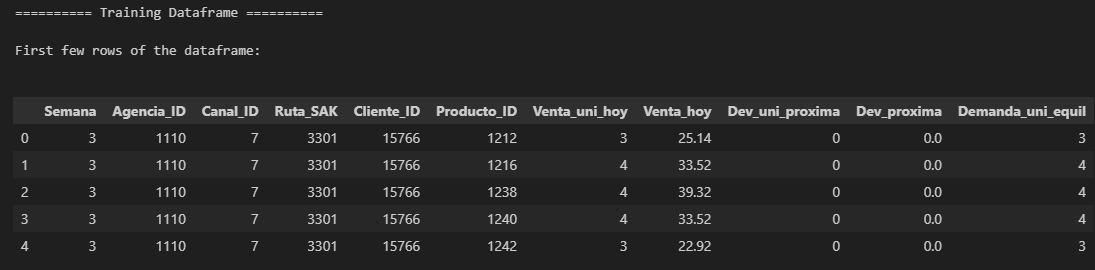
\includegraphics[width=0.9\textwidth]{images/train_df.png}
\caption{Train Dataframe}
\end{center}
\end{figure}

\begin{figure}[H] 
\begin{center}
\centering
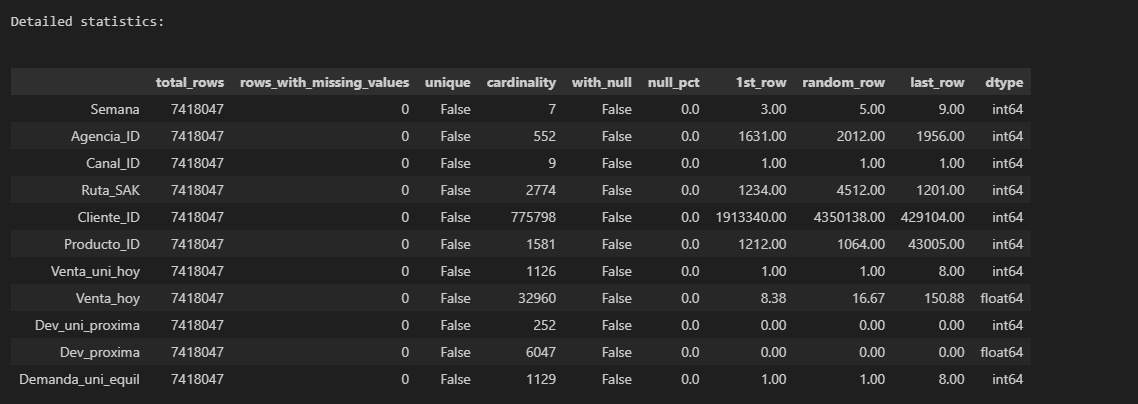
\includegraphics[width=0.9\textwidth]{images/descrip_train.png}
\caption{Description Train Dataframe}
\end{center}
\end{figure}

\begin{figure}[H]
\begin{center}
\centering
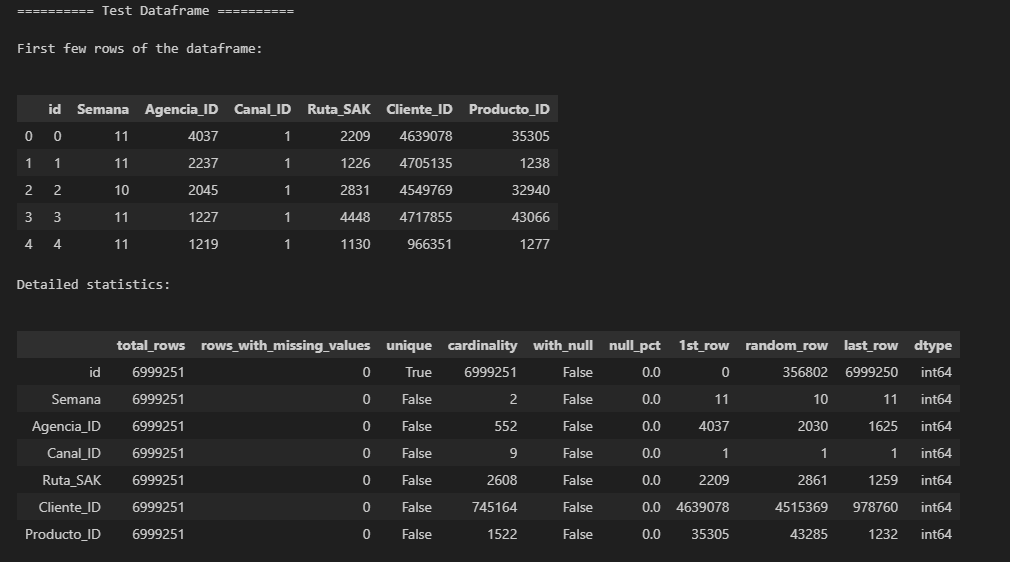
\includegraphics[width=0.9\textwidth]{images/test_df.png}
\caption{Test Dataframe}
\end{center}
\end{figure}

\begin{figure}[H] 
\begin{center}
\centering
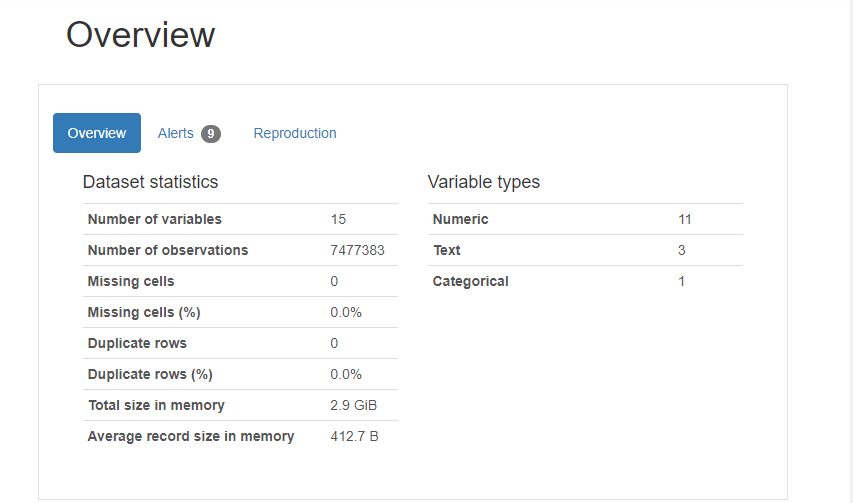
\includegraphics[width=0.9\textwidth]{images/train_ydata.png}
\caption{Ydata Profile Report Dataframe}
\end{center}
\end{figure}
    

\section{Data Preprocessing}
Invención de diodos emisores de luz azul que han permitido el desarrollo de fuentes de luz blanca y brillante de bajo consumo.\\\\
1) Su invención ha revolucionado la iluminación de las dos últimas décadas al permitir generar una luz blanca, brillante y barata.\\
2) Permitió crear lámparas led blancas, que emiten una luz brillante, son de larga duración y alta eficiencia energética.

\section{Feature Engineering}
Los científicos japoneses Isamu Akasaki, Hiroshi Amano y Shuji Nakamura han conseguido el premio Nobel de Física 2014 por haber inventado el led azul, una nueva fuente de luz eficiente, duradera y amigable con el medioambiente. 
Su invento permitió crear lámparas led blancas, que emiten una luz brillante, son de larga duración y alta eficiencia energética. Constantemente están mejorando, con mayores flujos luminosos (medidos en lúmenes) por unidad de energía eléctrica de entrada (medido en vatios). El registro más reciente es poco más de 300 lm/ W, en comparación con los 16 de las bombillas regulares y los cerca de 70 de las lámparas fluorescentes.

\section{Model Selection}
Cuando Akasaki, Amano y Nakamura produjeron haces brillantes de luz azul en semiconductores a principio de la década de 1990, desencadenaron una transformación fundamental en la tecnología de iluminación. Los diodos verdes y rojos ya se conocían desde hacía tiempo, pero sin el componte azul, las lámparas blancas no se podían crear. La invención del led azul tiene solo 20 años, pero ya ha contribuido a crear luz blanca de una forma nueva beneficiándonos a todos.

\section{Model Training}
El premio nobel otorgado a los autores mencionados anteriormente ha sido para dar reconocimiento a la gran labor que ellos hicieron por la creación de un nuevo invento de bajo consumo. La invención del led azul tiene solo 20 años, pero ya ha contribuido a crear luz blanca de una forma nueva beneficiándonos a todos.

\section{Model Evaluation}
ecuadoruniversitario.com  (2014). Quito – Ecuador. Isamu Akasaki, Hiroshi Amano y Shuji Nakamura reciben el Premio Nobel de Física 2014. Recuperado de: http://ecuadoruniversitario.com/ciencia-y-tecnologia/isamu-akasaki-hiroshi-amano-y-shuji-nakamura-reciben-el-premio-nobel-de-fisica-2014/

\section{Conclusions}
ecuadoruniversitario.com  (2014). Quito – Ecuador. Isamu Akasaki, Hiroshi Amano y Shuji Nakamura reciben el Premio Nobel de Física 2014. Recuperado de: http://ecuadoruniversitario.com/ciencia-y-tecnologia/isamu-akasaki-hiroshi-amano-y-shuji-nakamura-reciben-el-premio-nobel-de-fisica-2014/

SINC. (2014). Madrid – España. Premio Nobel de Física 2014 para los creadores del led azul. Recuperado de: https://www.agenciasinc.es/Noticias/Premio-Nobel-de-Fisica-2014-para-los-creadores-del-led-azul 

\end{document}
